\documentclass [a4paper, 11pt] {article}
\setlength\parindent{0pt}


\usepackage{amsmath}

\usepackage{blindtext}
\usepackage{graphicx}
\usepackage[table]{xcolor}
\usepackage{dcolumn}

% bibliography
\usepackage [style=bwl-FU, url=false, eprint=false]{biblatex}
\addbibresource{biblio.bib}

\setcounter{secnumdepth}{0}

\newcolumntype{L}{D{.}{.}{2,5}}

\begin{document}
% title description 
\title {\Huge Final Project \\
 \Huge Digital Tools for Finance }
\author {\huge Elena Ten 19-765-395, \\
	 	 \huge Elena Grigorenko 19-738-343}

\date {\huge 15.12.2020}



% create title
\maketitle
\thispagestyle{empty}

\newpage

\tableofcontents

\newpage

\section {Introduction}
The main objective of this report is to analyse the oil industry, focusing on the cost of capital and stock prices of the chosen companies. Nine biggest companies, representing the industry were chosen. \\
This report is aimed on the estimation of the cost of capital of the main players of the oil industry.\\
The first part of the report gives an overview of stock prices of the companies, including analysis, predictions, as well as returns rate and risks.\\
The second part of the report is dedicated to the estimation of the cost of capital.

\section {Stock Price Analysis}
The evaluation of the stock prices of the oil companies was carried out in Python.\\
Lukoil company was chosen as a benchmark to evaluate and compare the stock price performance relative to the competitors.\\
The analysis is focused on closing prices, to provide a better understanding of the stock performance. we analyse stocks using two key measurements: Rolling Mean and Return Rate.\\
As the first step we study the stock prices of Lukoil.


\subsection {Stock price of Lukoil}
First, we plot Lukoil time-series. Then, we would like to assess how the stock behaves compared to a short and longer term moving average of its price.
% insert LUKOIL MA
\begin{figure}[h]
\caption{Moving Average of Closing Price of PJSC Lukoil}
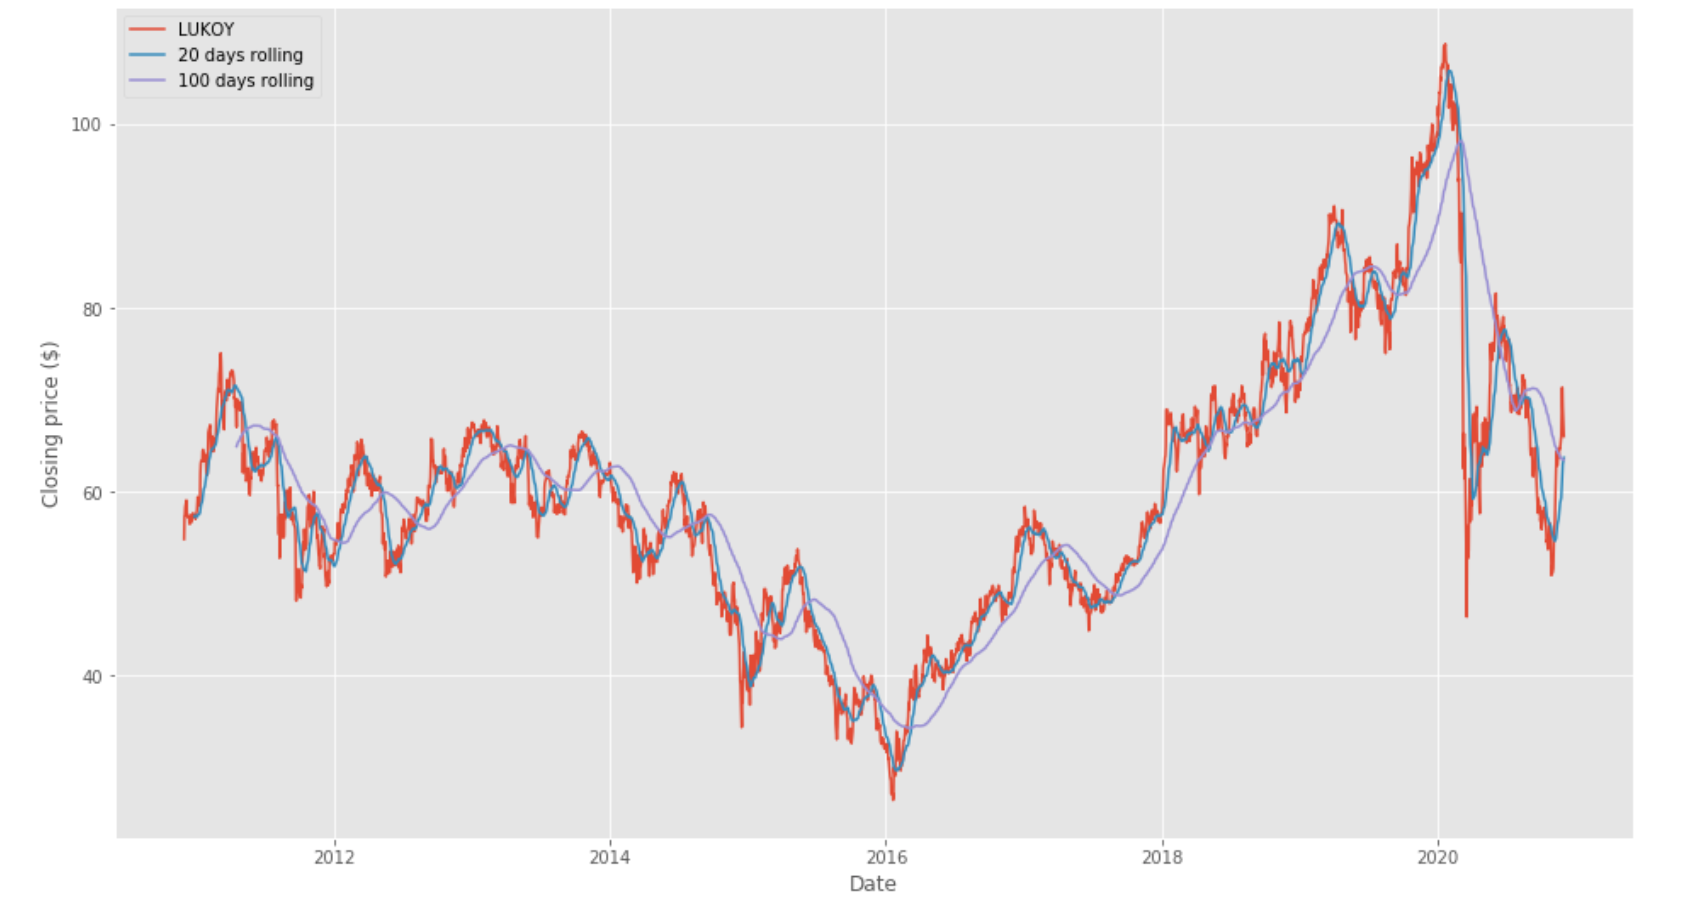
\includegraphics[height=6.5cm]{LUKOIL_MA}

\end{figure}

\clearpage

\subsection {Overview of Moving Averages of the industry}
For further analysis we decided to explore Moving Average of the companies, representing the industry.

% insert Industry_MA
\begin{figure}[h]
\begin{center}
\caption{Moving Average of Closing Price}
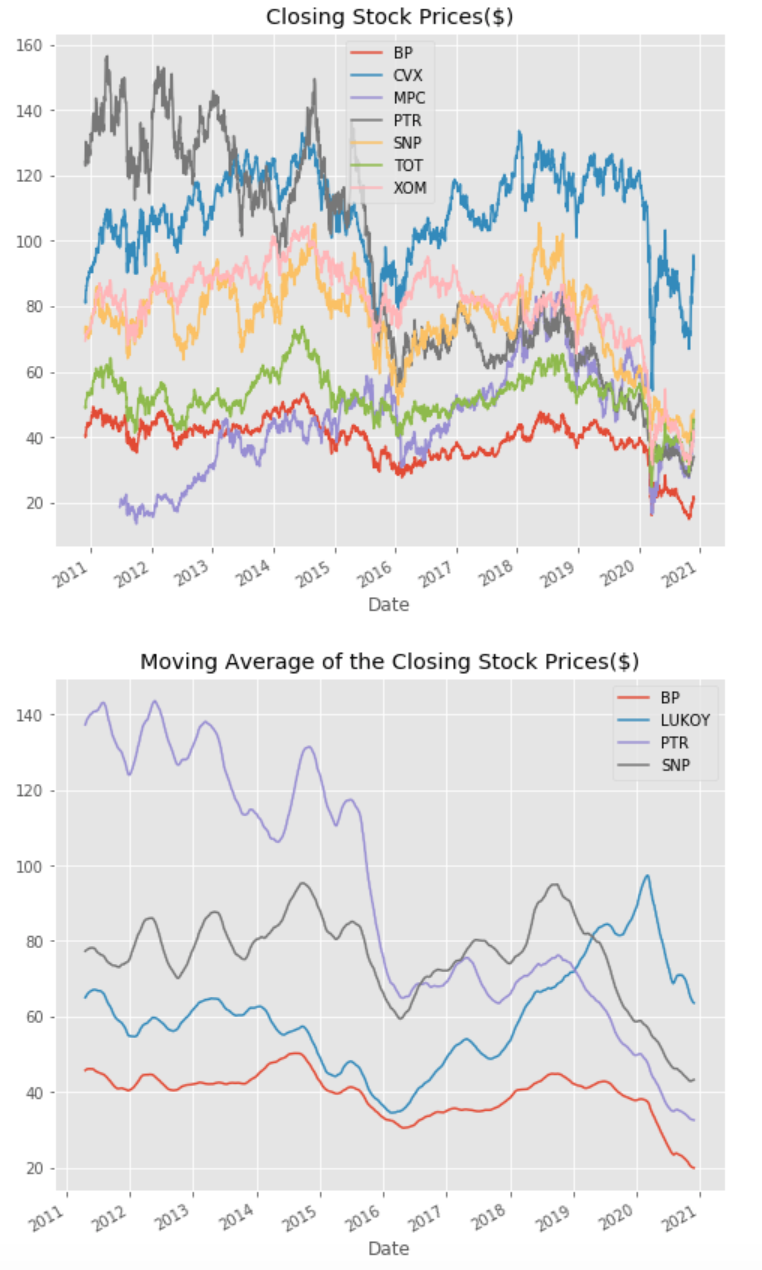
\includegraphics[height=15cm]{Industry_MA}
\label{fig:ma2}
\end{center}
\end{figure}

\clearpage

\subsection {Analysing Competitors Stocks}
In this section, we analyse on how one company performs compared to the competitor.  Based on the conducted an analysis, we conclude that there is no relationship between Lukoil returns and Royal Dutch Shell returns. On the other hand, there are positive correlations between Lukoil returns and BP return.

% insert Lukoil vs RDS
\begin{figure}[h]
\caption{Returns of Lukoil and Competitorsl}
\begin{center}
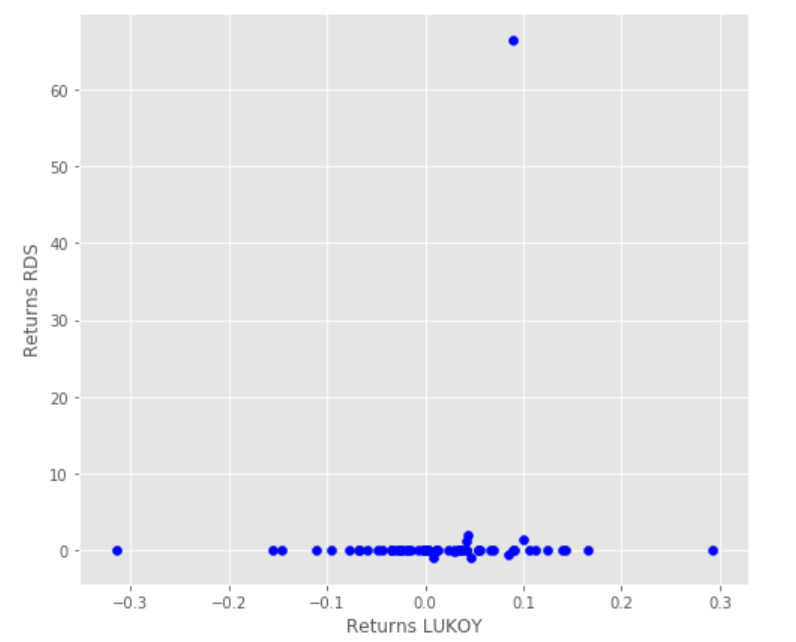
\includegraphics[scale=0.44]{Lukoil_RDS}
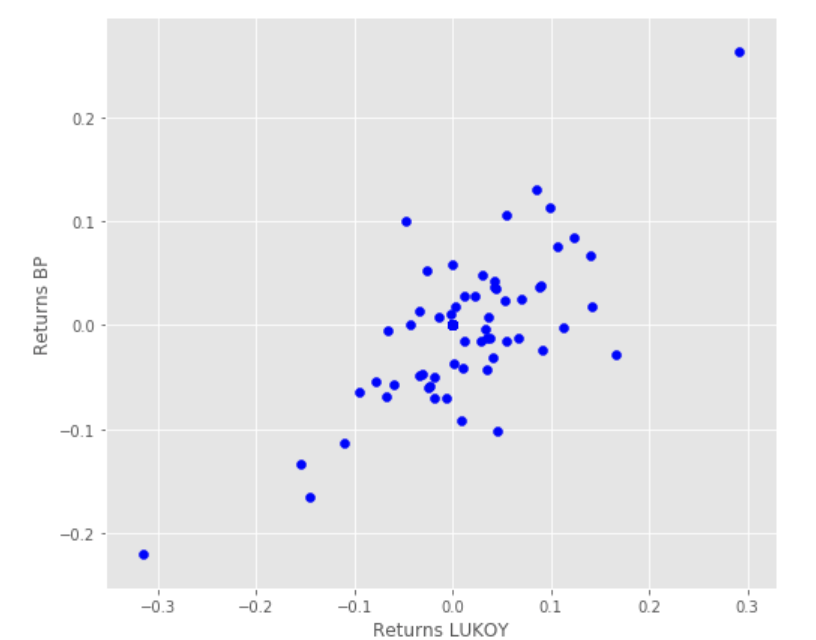
\includegraphics[scale=0.44]{Lukoil_BP}
\end{center}
\label{fig:scat1}
\end{figure}

To improve analysis we plot scatter matrix to visualise possible correlations, by running Kernel Density Estimate.

% insert scatter matrix
\begin{figure}[h]
\caption{Chart of risk and return}
\begin{center}
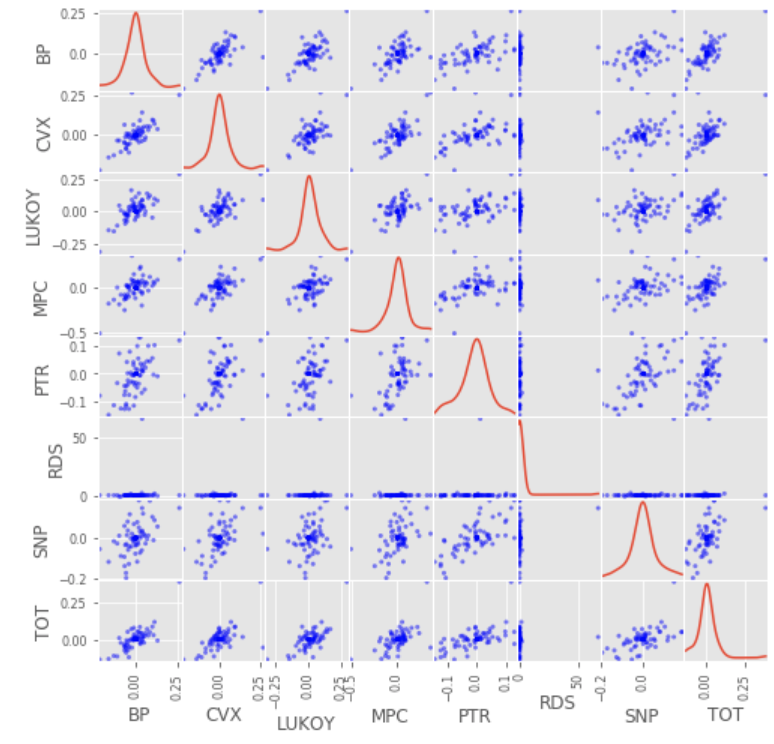
\includegraphics[scale=0.55]{matrix}
\label{fig:scat2}
\end{center}
\end{figure}
\clearpage

\subsection {Stocks Returns Rate and Risk}
Furthermore, we evaluate  risks and returns. In this case risks are represented by standard deviation of returns and returns are represented by average of returns.
Exclude RDS as it distorts the graph.\\

% insert scatter plot RR
\begin{figure}[h]
\caption{Risk vs Return}
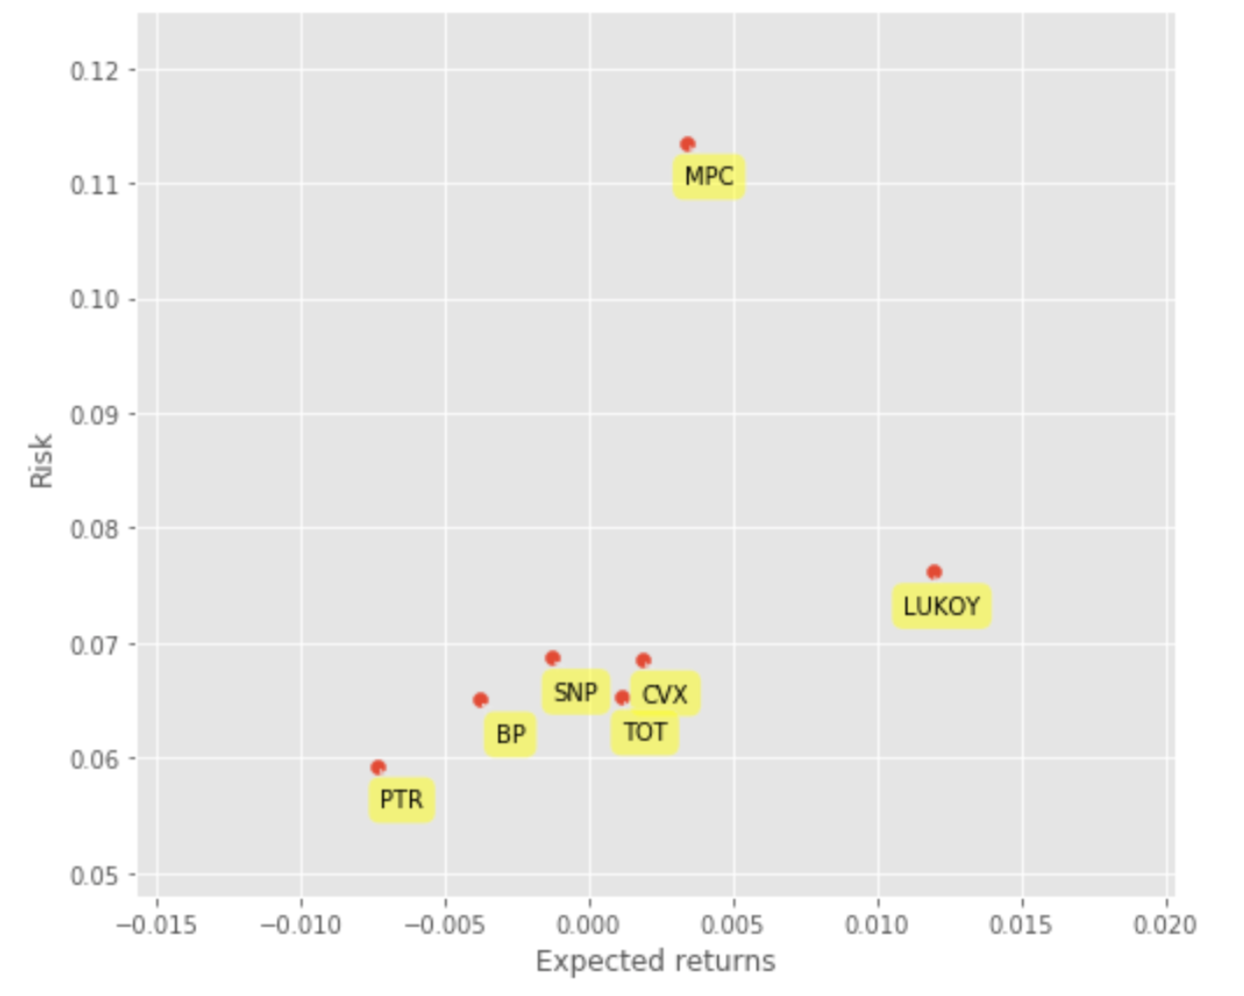
\includegraphics[scale=0.65]{return_risk}
\label{fig:scat4}
\end{figure}

\subsection {Stock Price prediction}
Finally we predict monthly stock prices of Lukoil for the next 2 years.

% insert predicted stock prices
\begin{figure}[h]
\caption{Predicted Stock Prices for Lukoil}
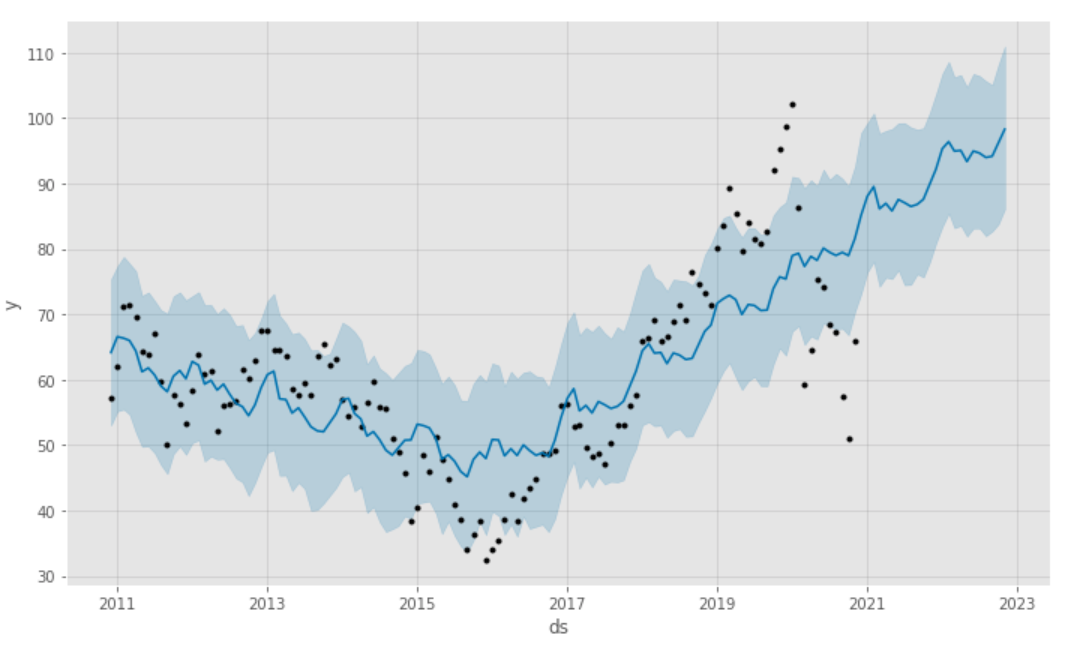
\includegraphics[scale=0.85]{Predicted}
\label{fig:graph}
\end{figure}
\clearpage

\section{Market}

% insert Companies statistics

\begin{table}[h]
\caption{Oil companies statistics\label{summary}} 
\begin{center}
\begin{tabular}{lLLLLLLLLL}
\hline\hline

\multicolumn{1}{l}{Statistics}&\multicolumn{1}{c}{ SNP }&\multicolumn{1}{c}{ PTR }&\multicolumn{1}{c}{  RDS }&\multicolumn{1}{c}{ BP }&\multicolumn{1}{c}{ XOM }&\multicolumn{1}{c}{ TOT }&\multicolumn{1}{c}{ CVX }\tabularnewline
\hline
Min.& \cellcolor{green!25} -0.0676 & \cellcolor{green!25} -0.0988& -0.1717& -0.1910& -0.1222& -0.1782 & -0.2212    \tabularnewline
1st Qu.&-0.0125  &-0.0142  &-0.0168  &-0.0172  &-0.0178  &-0.0127 &-0.0148   \tabularnewline
Median& \cellcolor{green!25} -0.0001  &-0.0023  &-0.0016 &-0.0031  &\cellcolor{red!25} -0.0045  &-0.0007 &-0.0020  \tabularnewline
Mean&-0.0005  &-0.0010  &-0.0011  &-0.0017  &-0.0017  &-0.0001  &-0.0004   \tabularnewline
3rd Qu.&0.0108 &0.0105  &0.0138  &0.0131  &0.0111  &0.0139 &0.0122  \tabularnewline
Max.&0.1026  &0.1490  & \cellcolor{green!25} 0.1967  & \cellcolor{green!25}0.2160  &0.1268 &0.1527  & \cellcolor{green!25} 0.2274   \tabularnewline
\hline
\end{tabular}\end{center}

\label{tab:comps}
\end{table}





% insert S&P plot
\begin{figure}[h]
\caption{Dynamics of S\&P Index}
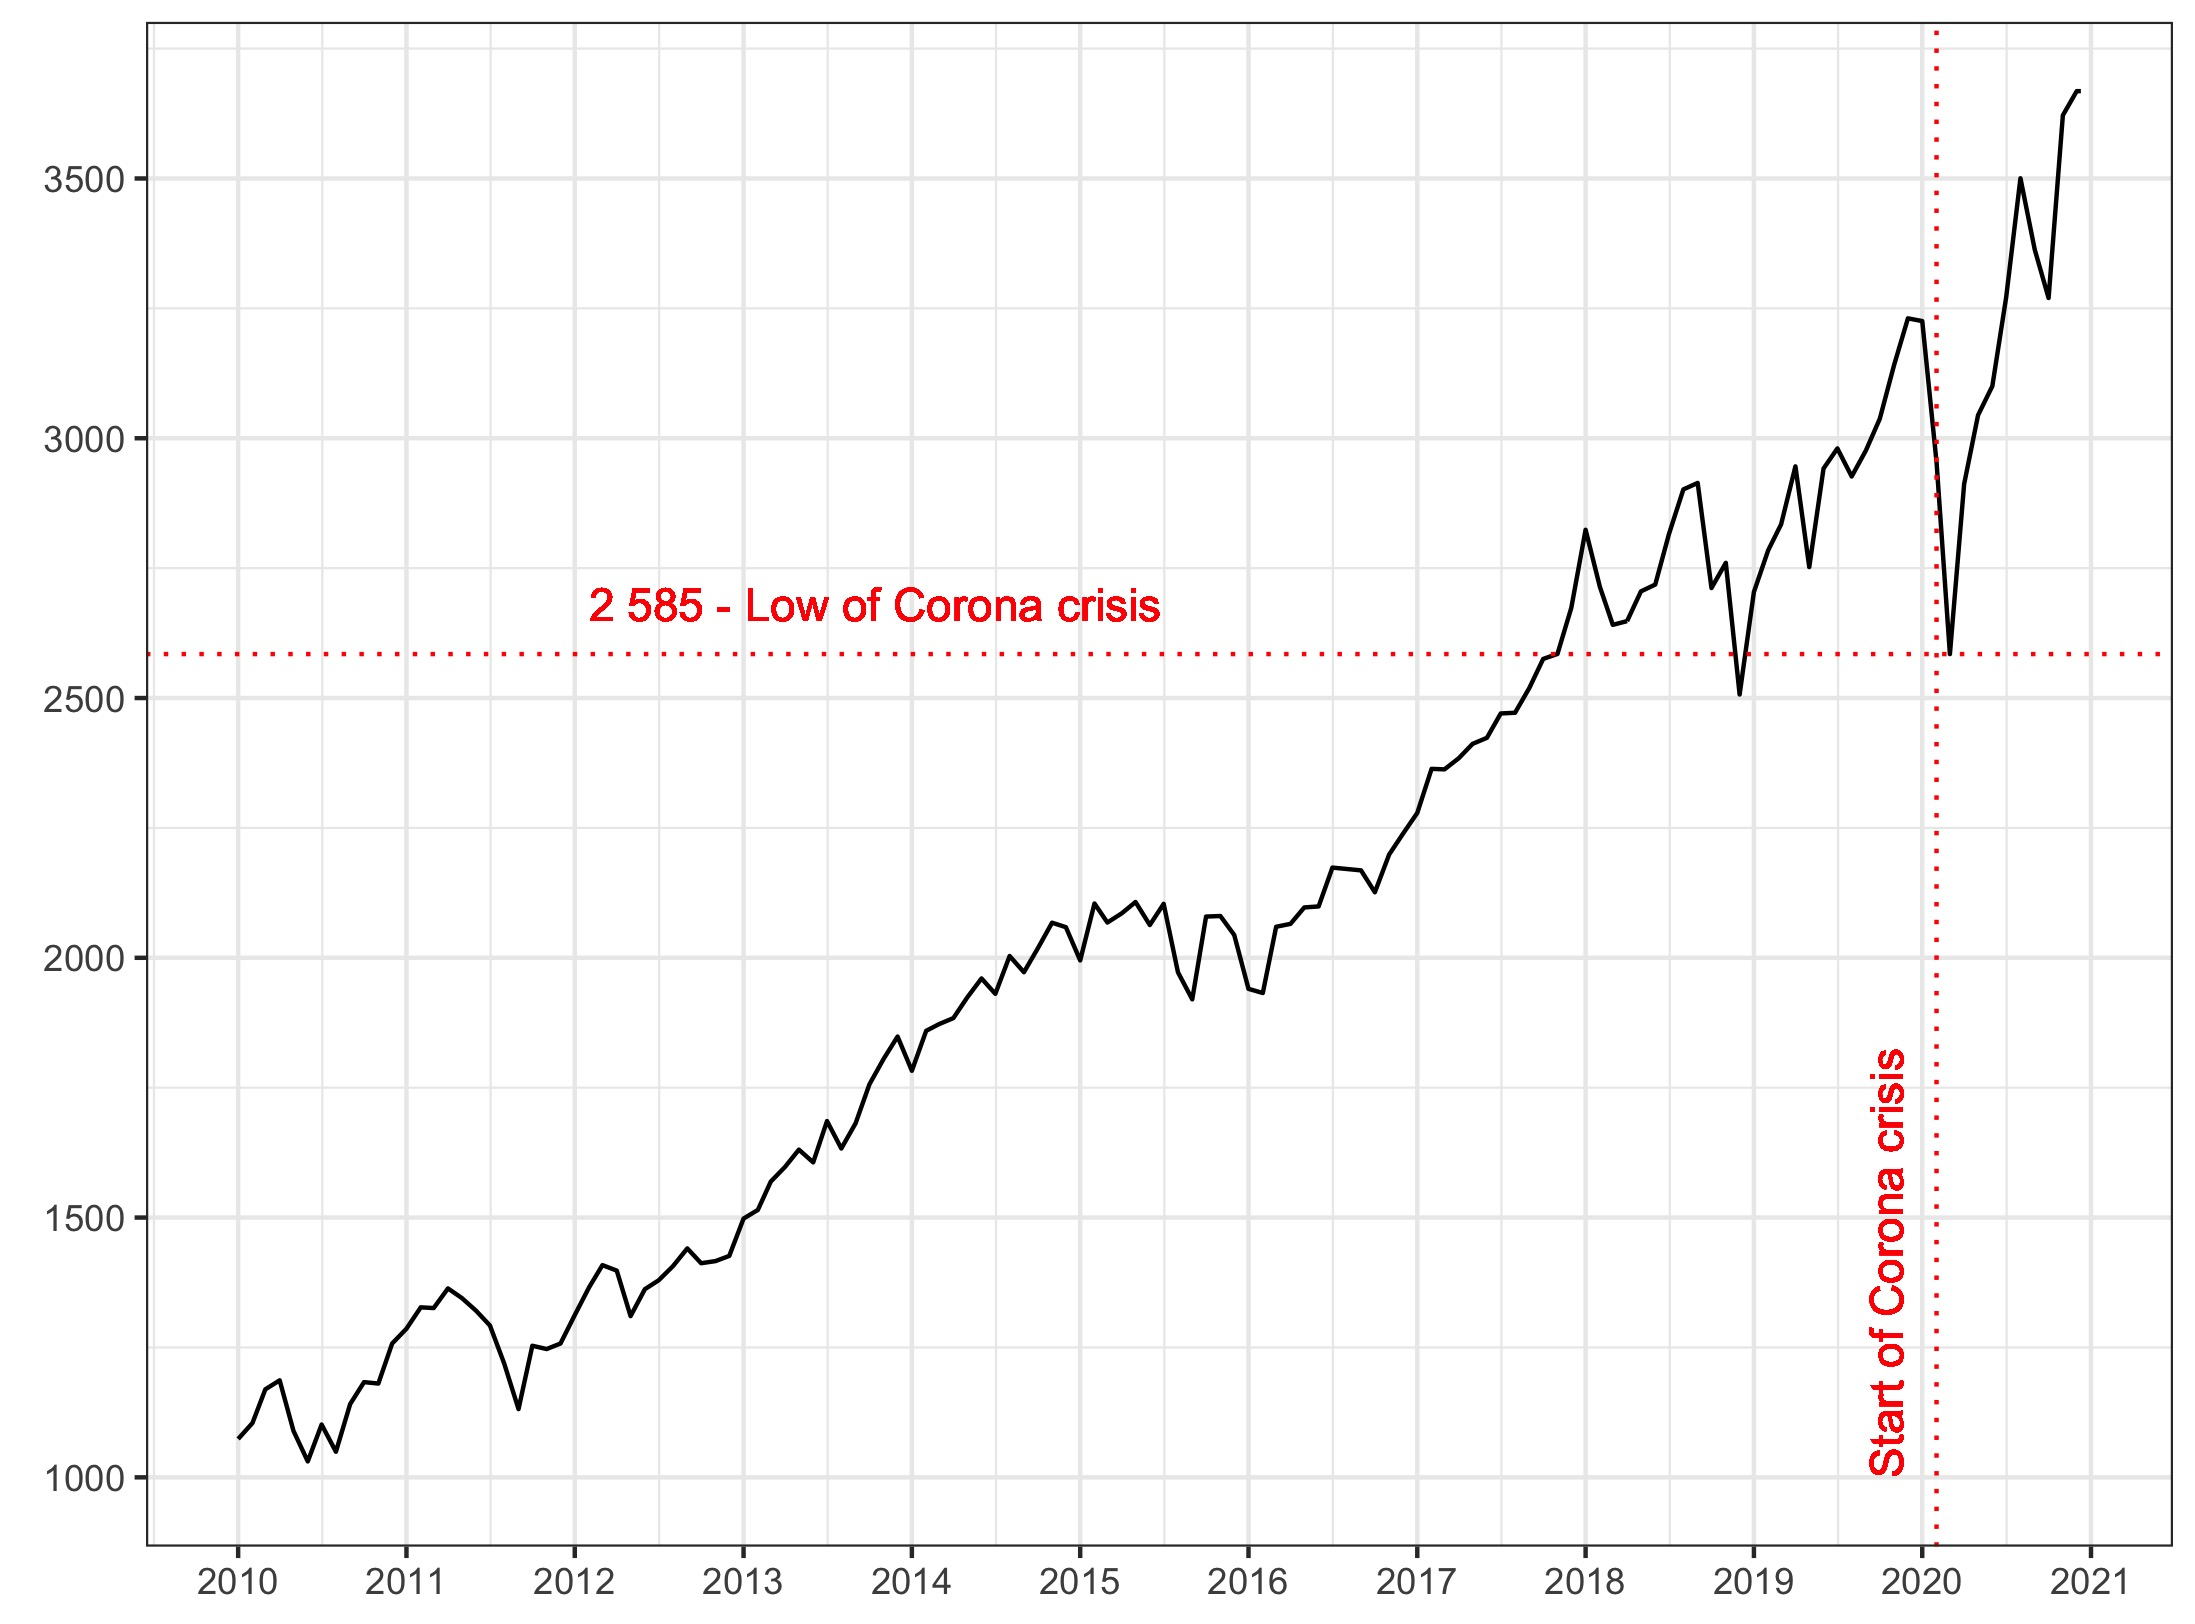
\includegraphics[scale=0.17]{sandp}
\label{fig:sandp}
\end{figure}


\clearpage
\section {Cost of Capital}
According to \cite{DamodaranDark} and \cite{BestPract}, one of the most prominents methods in calculating the cost of equity is the CAPM model, that is being implemented in the current research.

In this section we consider the type of the returns' distribution of several companies, as recommended by \cite{Fishman}.

% insert SNP hist plot
\begin{figure}[h]
\caption{Daily returns distribution of China Petroleum \& Chemical}
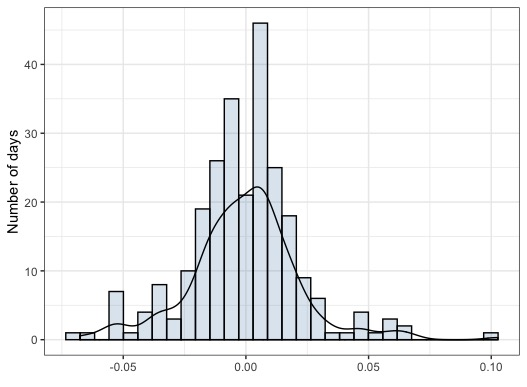
\includegraphics[scale=0.65]{snp_hist}
\label{fig:hist1}
\end{figure}

% insert LUKOIL hist plot
\begin{figure}[h]
\caption{Daily returns distribution of PJSC Lukoil}
\includegraphics[scale=0.65]{LUKOIL_hist}
\label{fig:hist1}
\end{figure}


\clearpage
\subsection {Risk-free rate}

According to \cite{Anderson}, for the estimation of risk-free rates we considered global risk-free rates (Figure ~\ref{fig:rf})

% insert r_f plot
\begin{figure}[!tbp]
\caption{Global risk free rates}
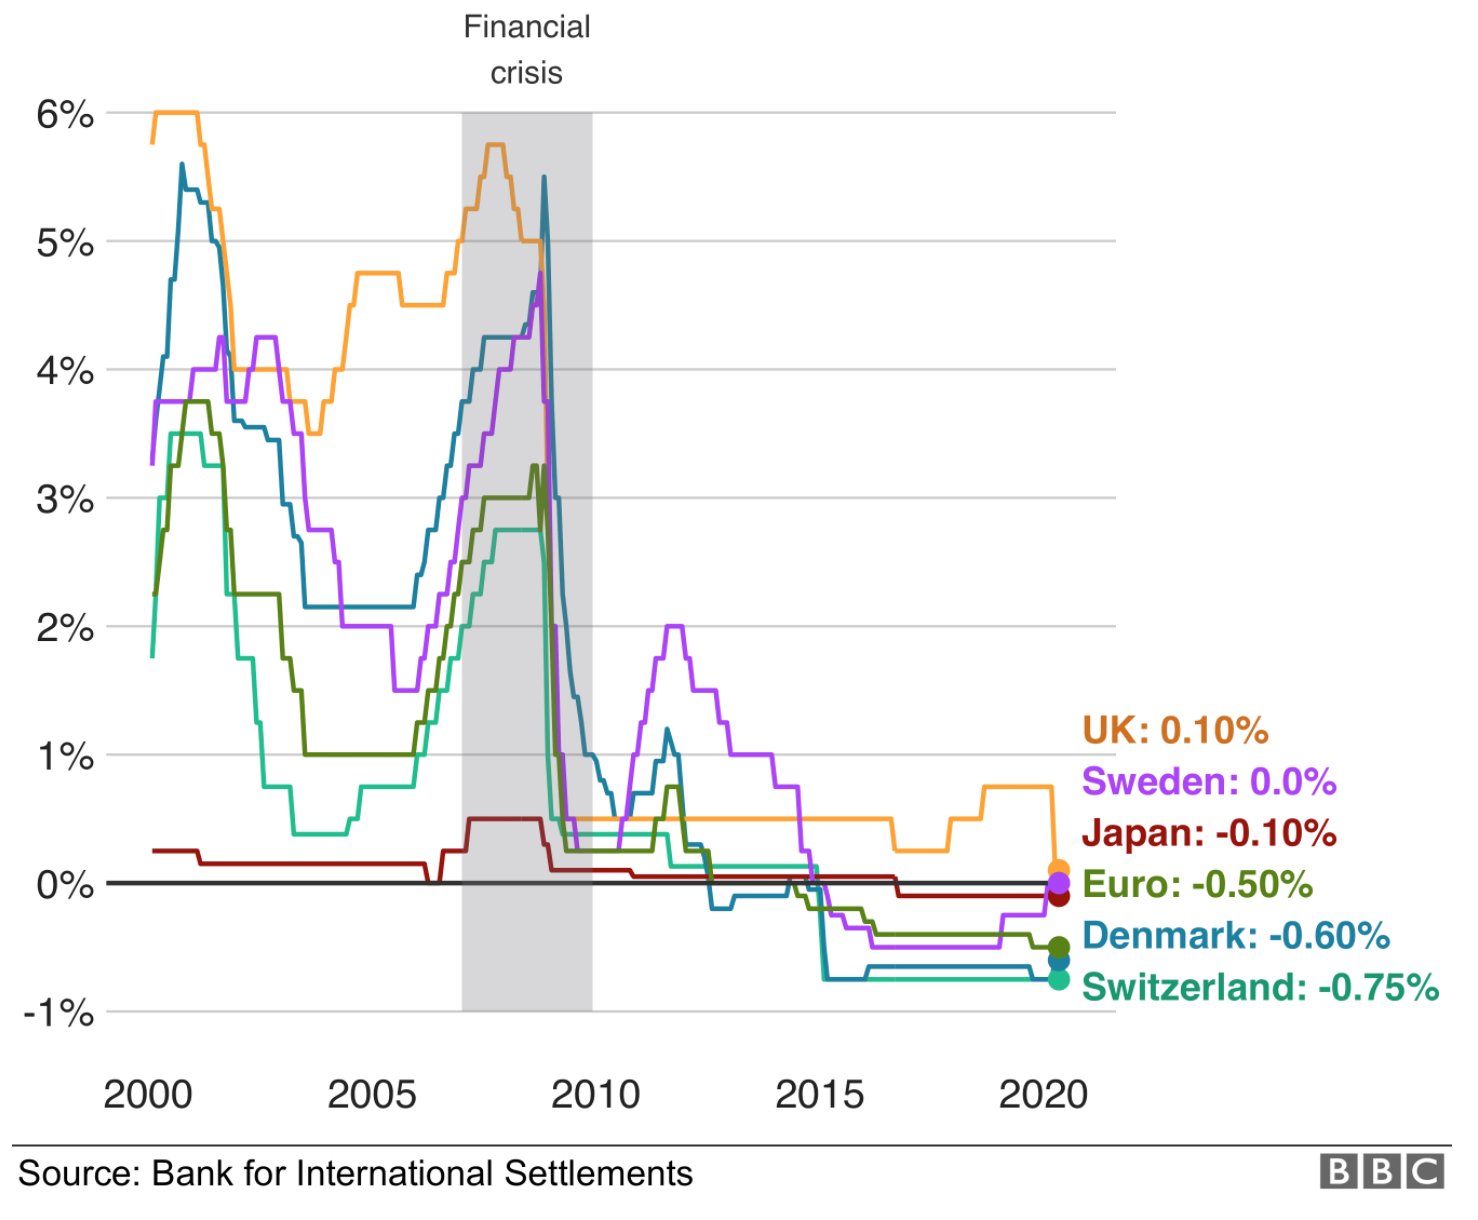
\includegraphics[scale=0.25]{risk_free}
\label{fig:rf}
\end{figure}

The risk free rate for the current project was accepted to be 0.

\clearpage
\subsection {Beta estimation}

Companies' beta coefficients were calculated, using the methodology, described by \cite{Casey}.\\
The 5 year time period was used for the estimation. The market index was represented by S\&P 500.\\
The results are presented in Table \ref{tab:beta}.\\

% insert beta table 
\begin{table}[!h]
\caption{Beta coefficients\label{beta}} 
\begin{center}
\begin{tabular}{llr}
\hline\hline
%\multicolumn{1}{l}{beta}&\multicolumn{1}{c}{comp_names}&\multicolumn{1}{c}{beta}\tabularnewline
%\hline
1&China Petroleum \& Chemical&$0.83$\tabularnewline
2&PetroChina&$0.97$\tabularnewline
3&Royal Dutch Shell PLC&$1.11$\tabularnewline
4&BP PLC&$1.09$\tabularnewline
5&Exxon Mobil Corp.&$1.02$\tabularnewline
6&Total SE&$1.07$\tabularnewline
7&Chevron Corp.&$1.20$\tabularnewline
8&Marathon Petroleum Corp.&$1.54$\tabularnewline
9&PJSC Lukoil&$0.97$\tabularnewline
\hline
\end{tabular}\end{center}
\label{tab:beta}
\end{table}

% insert beta plot
\begin{figure}[!h]
\caption{Beta Coefficients}
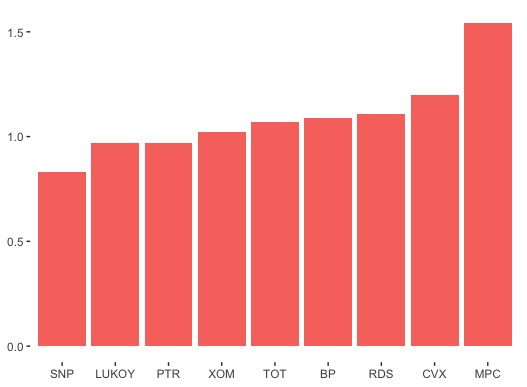
\includegraphics[scale=0.65]{beta_plot_bars}
\label{fig:beta}
\end{figure}

\clearpage
\subsection {Cost of Equity}

Cost of equity was calculated with the CAPM method, using the following formula:

$$ r_e = r_f + \beta (r_m - r_f)$$

The results of calculations are provided in Table \ref{tab:r_e}.

% insert r_e table
\begin{table}[!h]
\caption{Cost of Capital\label{r}} 
\begin{center}
\begin{tabular}{llr}
\hline\hline
%\multicolumn{1}{l}{r}&\multicolumn{1}{c}{comp_names}&\multicolumn{1}{c}{round.beta_df.beta...r_m..2.}\tabularnewline
%\hline
1&China Petroleum \& Chemical&$ \cellcolor{red!25} 0.15$\tabularnewline
2&PetroChina&$0.17$\tabularnewline
3&Royal Dutch Shell PLC&$0.20$\tabularnewline
4&BP PLC&$0.19$\tabularnewline
5&Exxon Mobil Corp.&$0.18$\tabularnewline
6&Total SE&$0.19$\tabularnewline
7&Chevron Corp.&$0.21$\tabularnewline
8&Marathon Petroleum Corp.&$ \cellcolor{green!25}0.27$\tabularnewline
9&PJSC Lukoil&$0.17$\tabularnewline
\hline
\end{tabular}\end{center}
\label{tab:r_e}
\end{table}



\clearpage
\subsection {Findings and Conclusion}
The conducted research allowed us to analyse oil industry from different aspects. \\
Having evaluated the stock prices, we conclude that the prices were at lowest in 2016 of all companies.
At the same time there is a possible correlation between returns on stock prices of oil companies. \\
The returns of RDS are dramatically higher compared to other companies. \\
Moreover, Marathon Petroleum stock prices has the highest risk and highest beta. On the other hand, Lukoil, chosen as benchmark company, has relatively low risk and beta and higher returns.\\
The prective model also showed expected growth in stock prices of Lukoil.

\clearpage
\newpage
\printbibliography [heading=bibintoc]

\end{document}
